\documentclass{article}

% if you need to pass options to natbib, use, e.g.:
% \PassOptionsToPackage{numbers, compress}{natbib}
% before loading nips_2016
%
% to avoid loading the natbib package, add option nonatbib:
% \usepackage[nonatbib]{nips_2016}

\usepackage[final]{nips_2016} % produce camera-ready copy
% to compile a camera-ready version, add the [final] option, e.g.:
% \usepackage[final]{nips_2016}

\usepackage[utf8]{inputenc} % allow utf-8 input
\usepackage[T1]{fontenc}    % use 8-bit T1 fonts
\usepackage{hyperref}       % hyperlinks
\usepackage{url}            % simple URL typesetting
\usepackage{booktabs}       % professional-quality tables
\usepackage{amsfonts}       % blackboard math symbols
\usepackage{nicefrac}       % compact symbols for 1/2, etc.
\usepackage{microtype}      % microtypography
\usepackage{blindtext}
\usepackage{caption}
\usepackage{subcaption}
\usepackage{graphicx}
\usepackage{float}
\usepackage[normalem]{ulem}
\useunder{\uline}{\ul}{}
\usepackage{graphicx}
\usepackage[table]{xcolor}

\title{Sentiment Classification for Movie Reviews}

% The \author macro works with any number of authors. There are two
% commands used to separate the names and addresses of multiple
% authors: \And and \AND.
%
% Using \And between authors leaves it to LaTeX to determine where to
% break the lines. Using \AND forces a line break at that point. So,
% if LaTeX puts 3 of 4 authors names on the first line, and the last
% on the second line, try using \AND instead of \And before the third
% author name.

\author{
  Adelina Badea\\
  s1728470\\
  \texttt{@ed.ac.uk} \\
  %% examples of more authors
  \And
  Daniel Biró\\
  s1618820\\
  \texttt{@ed.ac.uk} \\
 \And
  Azam Khan\\
  s1704037\\
  \texttt{@ed.ac.uk} \\
 \And
  Evan Moss\\
  s1715857\\
  \texttt{@ed.ac.uk}\\
}

\begin{document}

\maketitle

\begin{abstract}
This paper presents an implementation of machine learning methods to classify the sentiment for given phrases from movie reviews. Two feature representations are evaluated for the classifiers, these are TF-IDF, and Bag-of-Words (BOW). We found that BOW was the better performing of these two representations. The paper also presents an Exploratory Data Analysis. After thorough pre-processing and evaluation, we are able to achieve an accuracy of 65.78\% and 83.64\% when classifying over 5 classes and 2 classes respectively. This is achieved through a logistic regression model.
\end{abstract}

% \section{Instructions}

% The report should use this template and be 8 pages in length. Do not change the fontsize or layout. It should be compilable with pdflatex.

% Structuring the text as follows is likely useful, but definitely
% \emph{not} a requirement.

% \begin{itemize}
% \item Introduction
%   \begin{itemize}
%   \item description of the task/objective
%   \item relevant background and related previous work
%   \item explanation of the significance/relevance of the objective/task
%   \end{itemize}
% \item Data preparation
% \item Exploratory data analysis
% \item Learning methods
% \item Results
% \item Conclusions
% \end{itemize}

\section{Introduction}

%significance/relavance of the task
The rise of social media platforms has led to an increasing interest in sentiment analysis tasks. One application for sentiment analysis is as a tool for social media companies to protect its users from harassment and toxic comments. On microblogging sites such as Twitter or in the comments sections of content-sharing websites, text is often in the form of short messages. The classification of short texts is especially challenging because there is very little contextual information that can be extracted.

Due to the complexity of this task, many feature representations of text have been used in prior work to increase the accuracy of sentiment analysis systems. In this work, we investigate the use of two feature representations: bag of words (BOW) and term frequency-inverse document frequency (TF-IDF), and evaluate their effect on the performance of a model. We perform experiments on phrases from a corpus of movie reviews. These reviews were collected from the popular movie reviewing website Rotten Tomatoes. The curated dataset is called the Stanford Sentiment Treebank.

% Stanford Sentiment Treebank dataset
The Stanford Sentiment Treebank is comprised of 215,154 phrases labelled using the Amazon Mechanical Turk. Annotators were able to label a phrase with a degree of sentiment ranging from 'very negative' to 'very positive'. Experimenting on this dataset allows us to measure the performance of the model on very short phrases and full sentences. 

% Report structure
This report is structured as follows. In Section \ref{related work}, we discuss work previously carried out which relates to this field. Section \ref{data prep} details the steps taken to prepare and preprocess the data to be used for the experiments. In Section \ref{eda}, we present the results of exploratory data analysis performed on the dataset. In Section \ref{supervised}, a description of the various supervised machine learning methods used for the experiments is provided. Section \ref{results} provides details about the experiments and results.  

\section{Related Work}
\label{related work}

The Stanford Sentiment Treebank mentioned in the previous section was first introduced in \cite{socher2013recursive}. It is the first corpus with fully labelled parse trees, which the authors developed to train their novel model the Recursive Neural Tensor Network (RNTN) to capture the compositional effects of sentiment in language. 

The RNTN model is a Deep Learning approach based on Recurrent Neural Networks (RNNs), that performs computation on the input parse trees in a bottom up fashion. Since the trees are fully labelled the network's parameters can be adjusted at each sub-tree which all have an associated sentiment target value to be predicted. Values are propagated up to the root which represents the sentiment of the entire sentence.

With this model and data the authors have managed to outperform the then state of the art by almost 5\% in binary sentiment classification (around 85.4\% accuracy) and improve almost 10\% over the then common bag of features approach for fine grained sentiment classification of individual phrases (to around 80.7\%).

A more classical approach is presented in (\cite{paltoglou2010study}) where the authors took a support vector machine baseline and experimented with changing its weighting scheme. The initial model used binary unigram weighting which is simple but fails to capture the document representation appropriately.

In the field of Information Retrieval there are several classical document and term weighting schemes that work remarkably well for tasks such as content retrieval based on search engine queries. One of the most popular is term frequency inverse document frequency or tf-idf for short that was the focus of this study along with its variants.

The results show that using frequency based term weightings worked well in the sentiment classification domain as well, achieving better accuracy on movie review datasets than previous methods. Another important finding is that for reaching these high accuracies the weighting functions should scale sublinearly with the the number of times a term occurs in a document, and document frequency should be smoothed as well.

%https://www.aclweb.org/anthology/C14-1008.pdf
A slightly newer work improving on the performance of \cite{socher2013recursive} on the Stanford Sentiment Treebank is \cite{dos2014deep}. A different Deep Learning approach is taken by this work that is based on a Convolutional Neural Network (CNN). While RNNs are usually applied on sequence data, often in natural language processing due to their time-invariant recurrent nature, CNNs are most popular in computer vision tasks due to their position-invariant processing that can capture local features well. Nevertheless, CNNs have become more popular in language related tasks as well with some modification and this paper is an example of that.

% word2vec could need citation? 
The model used combines both word-level and character-level embeddings in the initial layers that build up to a sentence-level representation that can be scored. The word-level embeddings are learned in an unsupervised fashion via the popular word2vec tool. The character and sentence-level features are both computed via convolutional layers.

This setup has managed to outperform the RNTN model on the Stanford Sentiment Treebank, achieving 85.7\% accuracy on sentence level binary sentiment classification. The authors also evaluate their method on the Stanford Twitter Sentiment corpus where they achieve an accuracy of 86.4\%


\section{Data Preparation}
\label{data prep}

% Preprocessing


Each phrase within the dataset is labelled with a sentiment value in the range [0.0, 1.0]. This work attempts binary and multi-label classification. The mappings of the labels to the sentiment labels for both binary and multi-label analysis are shown in Tables 1 and 2.

\begin{table}[H]
\begin{minipage}{.48\linewidth}
\centering
\begin{tabular}{|c|c|}
\hline
\textbf{\begin{tabular}[c]{@{}c@{}}Sentiment Value \\ Intervals\end{tabular}} & \textbf{\begin{tabular}[c]{@{}c@{}}Sentiment \\ Label\end{tabular}} \\ \hline
{[}0.0, 0.2{]} & Very Negative \\ \hline
(0.2, 0.4{]}   & Negative      \\ \hline
(0.4, 0.6{]}   & Neutral       \\ \hline
(0.6, 0.8{]}   & Positive      \\ \hline
(0.8, 1.0{]}   & Very Positive \\ \hline
\end{tabular}%
\caption{Multi-label sentiments.}
\end{minipage}
\begin{minipage}{.48\linewidth}
\centering
\begin{tabular}{|c|c|}
\hline
\textbf{\begin{tabular}[c]{@{}c@{}}Sentiment Value\\ Intervals\end{tabular}} & \textbf{\begin{tabular}[c]{@{}c@{}}Sentiment\\ Label\end{tabular}} \\ \hline
{[}0.0, 0.55{]}                                                     & Negative                                                  \\ \hline
(0.55, 1.0{]}                                                       & Positive                                                  \\ \hline
\end{tabular}
\caption{Binary sentiments.}
\end{minipage}
\label{tab:my-table}
\end{table}

\subsection{Pre-processing}

Some pre-processing is carried out on the phrases. These are common techniques in natural langauge processing, and represent a way for the data to be standardised. Firstly, the data is ``case-folded", this is the process of converting all the words to the lower-case version of those words, this means that there can be comparison between the same words with different cases. For example ``FILM" and ``filM" both become ``film". Next, the words are ``tokenised", where the punctuation and formatting is removed, and we are left with only the words themselves. Finally, the words are ``stopped" and ``lemmatised". ``Stopping" is the processes of removing the most common words from the language from the text. This means that more focus is placed on important words rather than very common words like ``the" or ``and". For example, the phrase ``this film is superb" will be ``stopped" to become ``film superb", if ``this" and ``is" are stop words. ``Lemmatisation" is the process of coverting all forms of the same word to a single word, again to aid the comparison of phrases. For example, ``great", ``greater" and ``greatest" all become ``great. An example of a pre-processed very negative phrase and very positive phrase is shown in Table \ref{tab:pre-proc}.

\begin{table}[h]
    \centering
    \begin{tabular}{|c|c|}
        \hline
         \textbf{Sentiment} & \textbf{Pre-processed Phrase} \\
         \hline
         Very Positive (1.0) & `best film year far benchmark best picture contender measure'\\
         \hline
         Very Negative (0.0) & `bang head seat front cluelessness idiocy'\\
         \hline
    \end{tabular}
    \caption{Pre-processed positive and negative phrases}
    \label{tab:pre-proc}
\end{table}

% Dataset splits
After preprocessing, the dataset was split into training, validation and test sets. 20\% of the dataset was held out as a test set for estimating the generalisation performance. 

\begin{table}[H]
\centering
\begin{tabular}{|cc|}
\hline
Split       & \# Phrases \\ \hline
Training    & 152955 \\
Validation & 37000 \\
Test        & 47489 \\ \hline
\end{tabular}%
\caption{Dataset Splits.}
\label{tab:splits}
\end{table}

\section{Exploratory Data Analysis}
\label{eda}

% Word clouds

\begin{figure}[h]
    \centering
    \begin{subfigure}{0.49\textwidth}
        \centering
        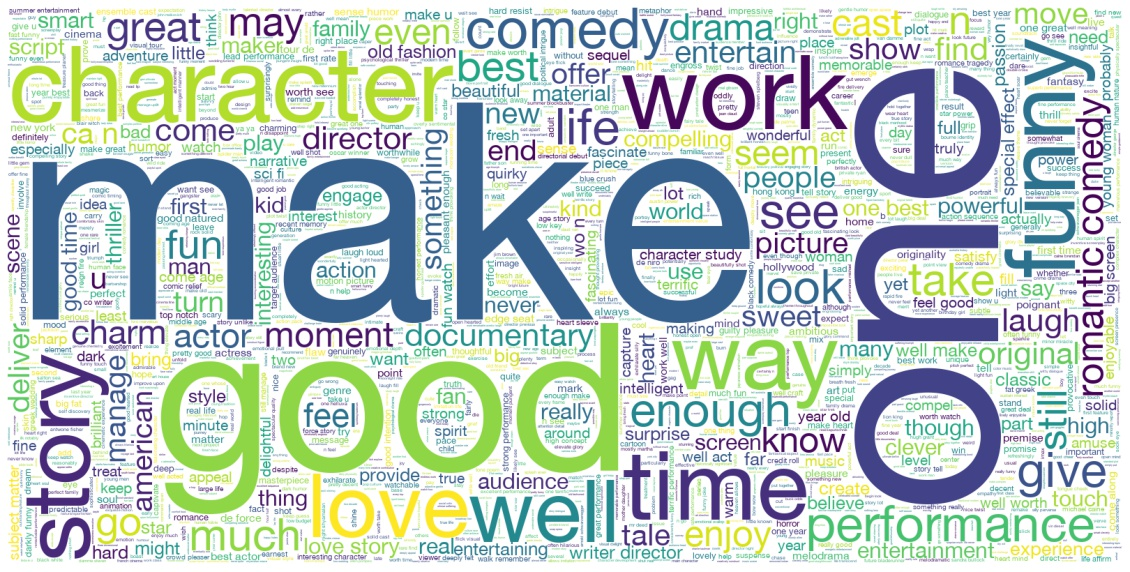
\includegraphics[width=\textwidth]{DME-template/figs/good_cloud.jpg}
        \caption{Word cloud for positive reviews. Sentiment values: (0.6-1.0].}
    \end{subfigure}
    \begin{subfigure}{0.49\textwidth}
        \centering
        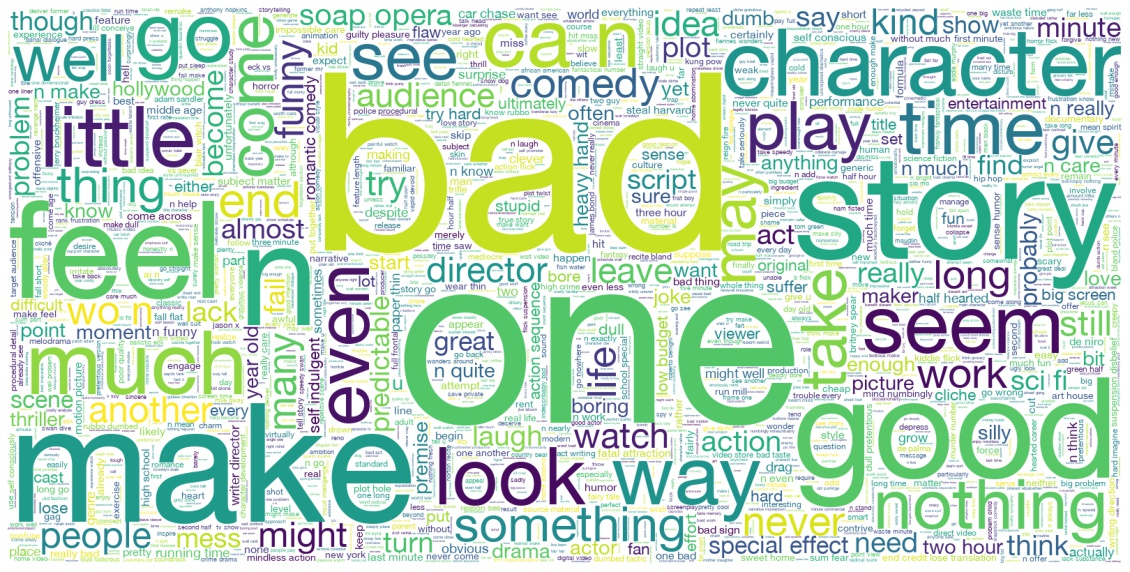
\includegraphics[width=\textwidth]{DME-template/figs/bad_cloud.jpg}
        \caption{Word cloud for negative reviews. Sentiment values: [0-0.4].}
    \end{subfigure}
    \caption{Word clouds for positive and negative reviews.}
    \label{fig:word_clouds}
\end{figure}

Before attempts were made at classification, exploratory data analysis was carried out in order to get an idea of the structure of the data. Through several visualisations, insights into the location, shape, and scale are found.

Firstly, there was analysis into the scale and the location of the data. Table \ref{tab:loc_scale} shows mean, median, mode and standard deviation of the data.

\begin{table}[h]
    \centering
    \begin{tabular}{c|c|c|c}
         \textbf{Mean} & \textbf{Median} & \textbf{Mode} & \textbf{Standard Deviation}  \\
         \hline
         0.513 & 0.5 & 0.5 & 0.176 \\
    \end{tabular}
    \caption{Location and scale measures of the data.}
    \label{tab:loc_scale}
\end{table}

Following this, it was decided to gain insight into the shape of the data. One way to measure this is to find the skewness of the data. The skewness of the data is $-0.0397$. This shows that the mass is concentrated slightly to the right of the distribution, with a longer left tail. This is negligable though, and should mean that the data is still symmetrical. Furthermore, the kurtosis can be found, which measures how often the value is considerable larger or smaller than the standard deviation, or `how heavy the tails' of the distribution are. The kurtosis of the data is $-0.035$. Figure \ref{fig:skewness} shows the density of the data, this confirms that the data is symmetric.

% Skewness
%Maybe add regions of sentiment
% \begin{figure}[h]
%     \centering
%     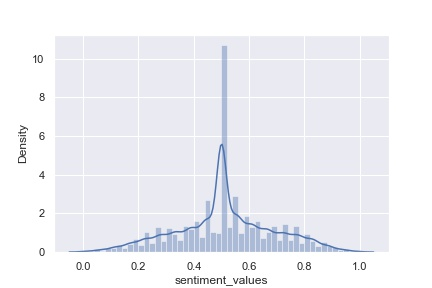
\includegraphics[width=0.7\textwidth]{DME-template/figs/sentiment_values_density.jpg}
%     \caption{Density plot of sentiment values.}
%     \label{fig:skewness}
% \end{figure}

% \begin{figure}[h]
%     \centering
%     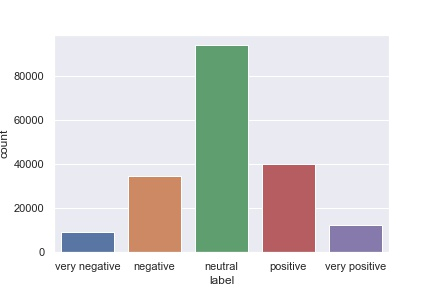
\includegraphics[width=0.75\textwidth]{DME-template/samples_training.jpg}
%     \caption{Class imbalance for ``neutral" label.}
%     \label{training_samples}
% \end{figure}

\begin{figure}[h]
\centering
\begin{minipage}{.5\textwidth}
    \centering
    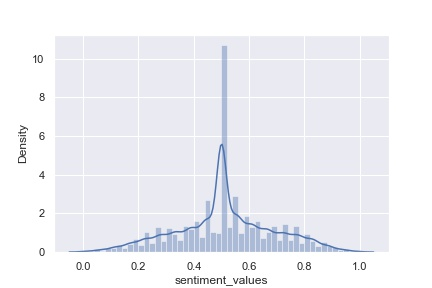
\includegraphics[width=\textwidth]{DME-template/figs/sentiment_values_density.jpg}
    \caption{Density plot of sentiment values.}
    \label{fig:skewness}
\end{minipage}%
\begin{minipage}{.5\textwidth}
    \centering
    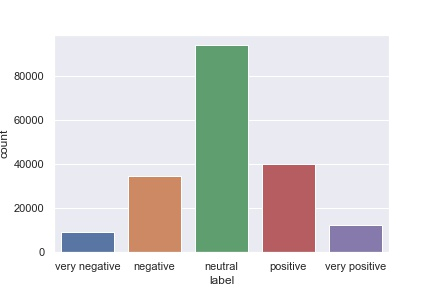
\includegraphics[width=\textwidth]{DME-template/samples_training.jpg}
    \caption{Class imbalance for ``neutral" label.}
    \label{training_samples}
\end{minipage}
\end{figure}



Finally, it was decided to get an insight into the phrases themselves, with particular focus on words and phrases that occur in positive and negative reviews. Figure \ref{fig:phrase_words} shows the number of words that appear in each of the classes.

% Class distribution
\begin{figure}[h]
    \centering
    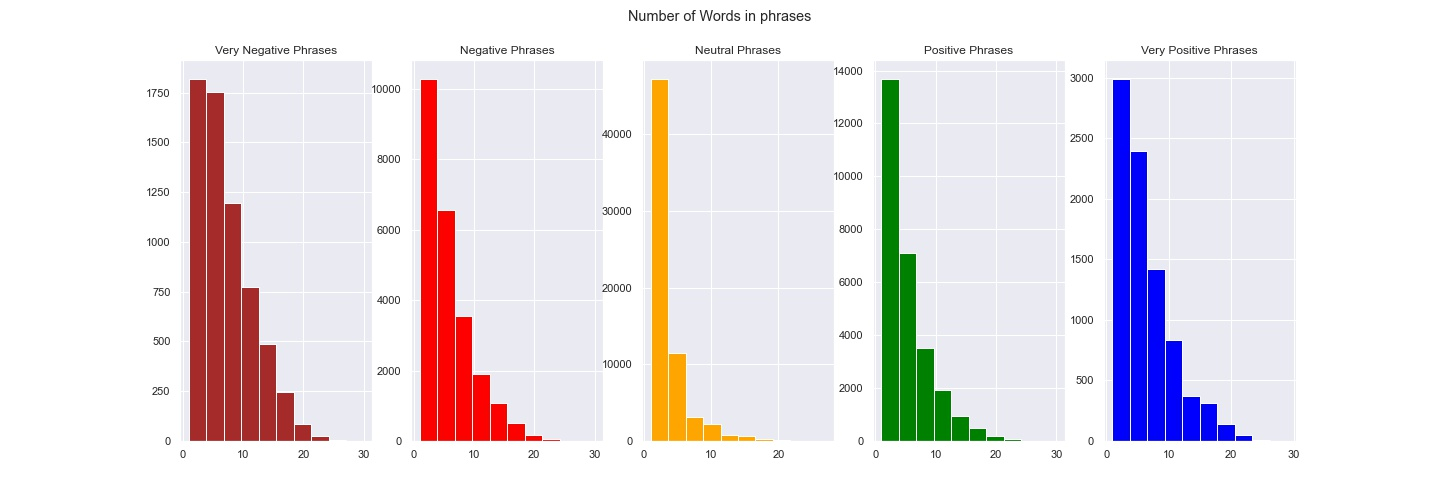
\includegraphics[width=\textwidth]{DME-template/figs/number_words.jpg}
    \caption{Number of Words in Phrases.}
    \label{fig:phrase_words}
\end{figure}

Next, a treemap is shown of the top 10 words from phrases with positive or negative sentiment in Figure \ref{fig:common_words}. These figures have had the words `film' and `movie removed, as they were so common in each. It could be an idea that in pre-processing, these words are removed as ``stop-words".

% Common words
% Could change to mean word length
\begin{figure}[h]
    \centering
    \begin{subfigure}{0.49\textwidth}
        \centering
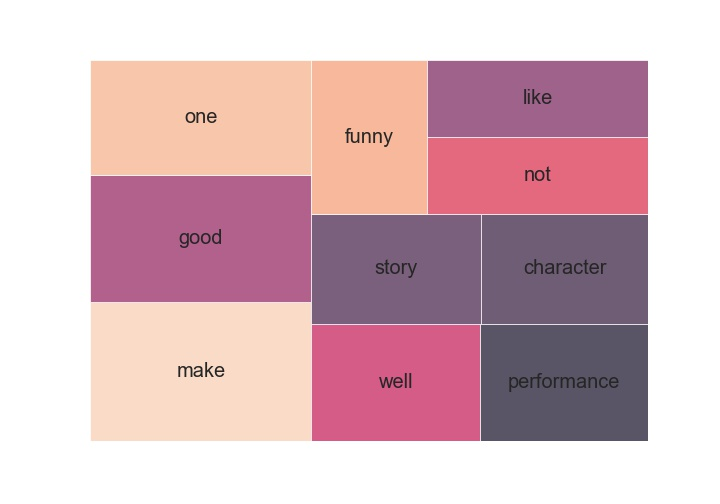
\includegraphics[width=\textwidth]{DME-template/figs/common_good.jpg}
        \caption{Most common words in positive reviews.}
    \end{subfigure}
    \begin{subfigure}{0.49\textwidth}
        \centering
        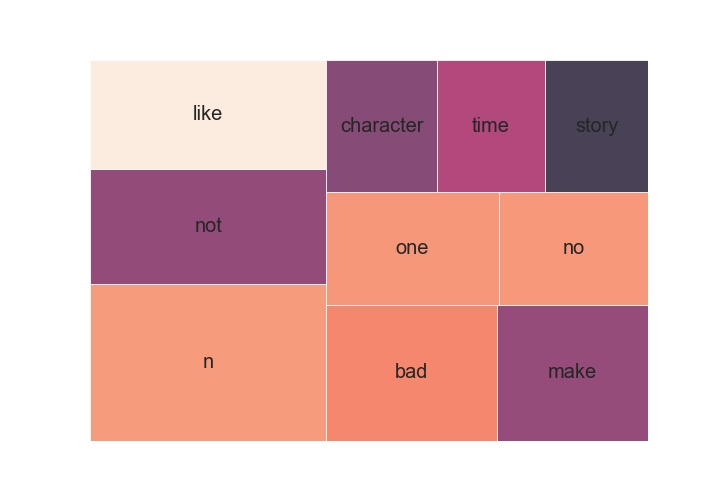
\includegraphics[width=\textwidth]{DME-template/figs/common_bad.jpg}
        \caption{Most common words in negative reviews.}
    \end{subfigure}
    \caption{Top 10 most common words in either positive (or very positive) or negative (or very negative) reviews.}
    \label{fig:common_words}
\end{figure}

Finally, an analysis into the most common word-level tri-grams is carried out. This should give us an idea of some common 3 word pairs that appear in each of the reviews. Figure \ref{fig:tri-grams} shows these results for reviews labelled ``very positive" and ``very negative". The top examples in each of these classes are ``tour de force" and ``indescribably bad movie" and they both offer particularly good examples of tri-grams representing common phrases you would associate with very positive or negative reviews. Other interesting examples include "one year best" - since the data has been pre-processed, this phrase is likely to have been "one of the year's best" or some similar phrase. ``Numbingly indescribably bad" and ``meaningless vapid devoid" are also particularly descriptive tri-grams that are common within the negative reviews. 

% Tri-grams
\begin{figure}[H]
    \centering
    \begin{subfigure}{0.49\textwidth}
        \centering
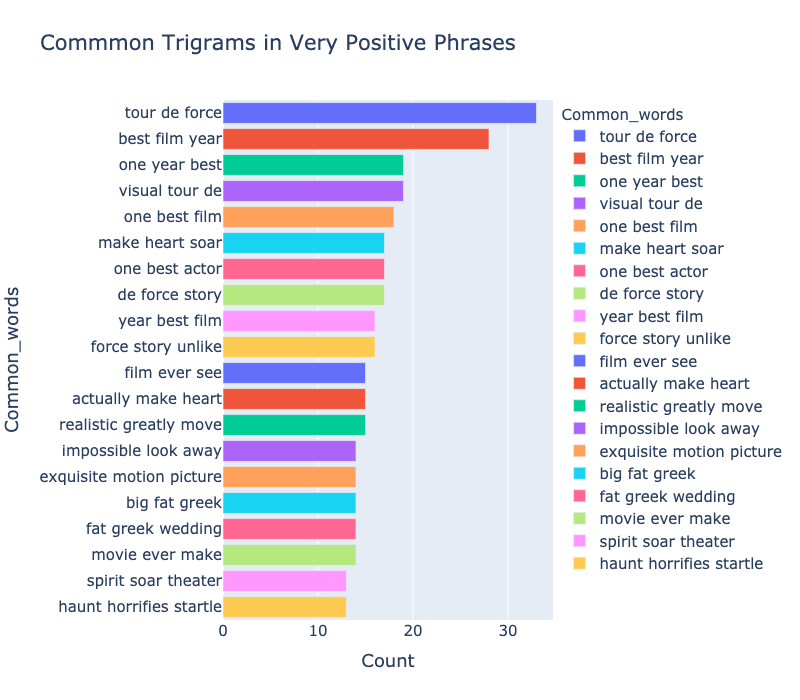
\includegraphics[width=\textwidth]{DME-template/figs/good_tri_grams.png}
        \caption{Most common tri-grams in very positive reviews.}
    \end{subfigure}
    \begin{subfigure}{0.49\textwidth}
        \centering
        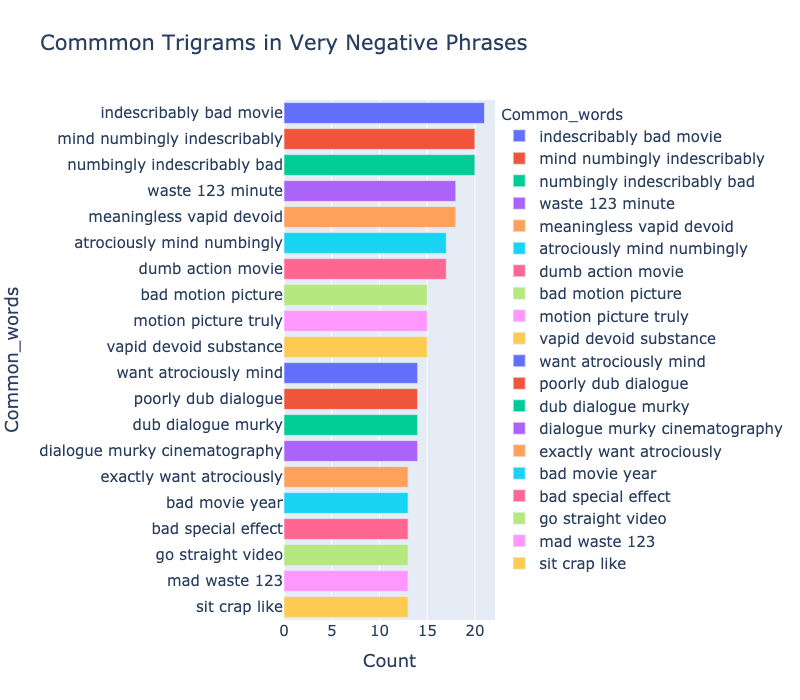
\includegraphics[width=\textwidth]{DME-template/figs/bad_tri_grams.png}
        \caption{Most common tri-grams in very negative reviews.}
    \end{subfigure}
    \caption{Caption}
    \label{fig:tri-grams}
\end{figure}



\section{Learning Methods}
\label{supervised}

To choose a best-performing model, a `Two Times Hold-out' approach was employed. The performances of the various supervised learning methods and feature representations were evaluated on a validation set containing 37000 labelled phrases (20\% of the training set). The model that is able to achieve the best accuracy/f1-score was then trained on the union of the training and validation sets. The performance is evaluated on the test set and further analysed.

%Bag of words vs TF-IDF

\subsection{Logistic Regression}

Linear Regression is a standard used supervised learning algorithm for label classification, where the framework uses linear combinations of the processed movie reviews to output the class prediction. For binary classification, where it determines whether a review is ’positive’ or ‘negative’, it uses a\textit{ sigmoid activation function}, while for the fine-grained sentiment classification is applying a \textit{softmax function}. The output is represented by the index with the highest value as the class label. While the L2 regularisation is applied by default, we choose a 'lbfgs' solver for optimising logistic regression’s loss.

Before feeding our training data to the network, we converted the corpus into features using two approaches. We fit the model to both TF-IDF (term frequency-inverse document frequency) and BOW (bag-of-words) representations and compare the results to observe how feature scaling impacts our model's learning performance. From the classification reports, we can see that Logistic Regression achieved the highest precision in the negative (0.71) and neutral (0.60) classes and the highest accuracy among the implemented models.

\subsection{Linear SVM}

Support Vector Machines are known to perform well on sentiment classification. However, its performance is highly influenced by the used kernel function, which is applied to find the optimal hyperplane separating the data points. Due to the ability to project the input data into a higher dimensional vector space, in most classification processes, SVMs can handle imbalanced class frequencies.

We integrated a Linear SVM architecture, where a 'hinge' loss function with a stochastic gradient descent optimiser was used. To boost the generalisation performance, we used different slack penalties, aiming to find the optimal one. We ran the model on both the TF-IDF and BOW representations of the training corpus, learning that the latter yields relatively higher performance, reaching an accuracy of  81 \% on the binary classification task and 60\% on multi-labels.

\subsection{Random Forest}

Random Forest comprises multiple decision trees, one for each training entry. We integrated a baseline version of the classifier, which was trained on the BOW representation of the training collection. While its training time was significantly higher than the rest of the implemented supervised classifiers, it showed effective results in generalisation and handling the unbalanced dataset, as depicted in the Results chapter.

\subsection{Long Short-Term Memory}
We investigated the use of a deep learning method for this task. A Long Short-Term Memory (LSTM) model was used.

LSTM is a variant of recurrent neural networks (RNN). These are neural networks that use sequential data, making them common for natural language processing and language translation tasks. 

The neural net (NN) architecture of the implemented model is as follows: The input to the NN is the padded vector. The first layer is an embedding layer that converts a sequence of words into a sequence of vectors. After training, similar words are given similar values. The second layer is a dropout layer. The third layer is an LSTM layer with 100 recurrent units and uses a dropout rate of 0.1. The output layer is a fully connected layer with a single output for each of the labels.

The model was trained with various batch sizes and LSTM units to maximise the accuracy on the validation set. In the end, a batch size of 32 was chosen and 100 LSTM units. For binary classification, $binary\_crossentropy$ was used as the loss function, and for multi-label classification, $categorical\_crossentropy$ was used. We trained for 5 epochs. 

\subsection{Unsupervised Learning Methods}
We also tried using unsupervised clustering for this task. These methods involve iteratively building neighbourhoods of samples that are similar to each other without using any labels. A distance metric is used to evaluate the similarity and clusters of data are formed based on this. The number of clusters to be found is usually a hyperparameter of clustering algorithms.

The most widespread and convenient method is K-Means clustering, we applied this to our data. Two clusters were  defined in an attempt to classify either 'positive' or 'negative' sentiment. This produced an accuracy of 62\% and an f1-score of 0.525. 

Other clustering methods based on different methods were experimented with as well but unfortunately without getting results. Many of the methods available in packages such as scipy do not work with sparse matrices (due to the distance metrics employed and their computation methods), these required a prohibitive amount of memory to process our data. Some methods like Spectral and Birch clustering can work with sparse matrices (the underlying distance calculation is similar to K-means in these cases) but still take relatively lot of time and memory to compute, therefore we struggled to run them locally. A possible future direction of work would be evaluating these methods on a cluster. 

\section{Results}
\label{results}

The results of the various models are presented in Table \ref{tab:val_results_5} for 5-class prediction, and Table \ref{tab:val_results_binary} for binary classification.

\begin{table}[H]
\centering
\begin{tabular}{|c|cccc|}
\hline
Classifier                    & Precision & Recall  & F1-Score & Accuracy \\ \hline
\cellcolor[gray]{.8} Logistic Regression w/ BOW & \cellcolor[gray]{.8}63.58\%   & \cellcolor[gray]{.8}64.97\% & \cellcolor[gray]{.8}63.50\%  & \cellcolor[gray]{.8}64.97\%  \\
Logistic Regression w/ TF-IDF & 61.80\% & 63.09\% & 60.50\%  & 63.09\%  \\
SVM w/ BOW                    & 60.44\%   & 61.70\% & 58.20\%  & 61.70\%  \\
SVM w/ TF-IDF                 & 53.38\%   & 52.69\% & 41.94\%  & 52.69\%  \\
Random Forest w/ BOW                    & 62.95\%   & 63.87\% & 63.24\%  & 63.87\%  \\
LSTM                          & 63.36\%   & 64.43\% & 63.32\%  & 64.43\%  \\ \hline
\end{tabular}
\caption{Evaluation metrics for 5-class prediction on validation set.}
\label{tab:val_results_5}
\end{table}
\begin{table}[H]
\centering
\begin{tabular}{|c|cccc|}
\hline
Classifier                    & Precision & Recall  & F1-Score & Accuracy \\ \hline
Logistic Regression w/ BOW  \cellcolor[gray]{.8}  & \cellcolor[gray]{.8} 83.10\%  &\cellcolor[gray]{.8} 83.22\% & \cellcolor[gray]{.8} 82.92\%  &\cellcolor[gray]{.8} 83.22\%  \\
Logistic Regression w/ TF-IDF & 82.43\%   & 82.49\% & 82.08\%  & 82.49\%  \\
SVM w/ BOW                    & 81.13\%   & 80.39\% & 79.30\%  & 80.39\%  \\
SVM w/ TF-IDF                 & 77.01\%   & 73.40\% & 69.41\%  & 73.40\%  \\
Random Forest w/ BOW                    & 81.57\%   & 81.69\% & 81.32\%  & 81.69\%  \\
LSTM                          & 80.77\%          & 80.89\%         & 80.46\%          & 80.89\%          \\ \hline
\end{tabular}
\caption{Evaluation metrics for binary classification on validation set.}
\label{tab:val_results_binary}
\end{table}


The validation results show that using TF-IDF instead of simple BOW only made the results deteriorate substantially, in some cases by double digit percentage values.

In Figure 7, we present the confusion matrices for the best and worst-performing models when performing binary classification. We observe that in both cases that `positive' is misclassified very often.

Figure 8 shows the confusion matrices of best and worst-performing models when performing 5-label sentiment classification. It is observed that both models struggle to classify `Positive' correctly. However, the logistic regression model is able to more accurately classify the 'Very Negative' label.

\begin{figure}[H]
    \centering
    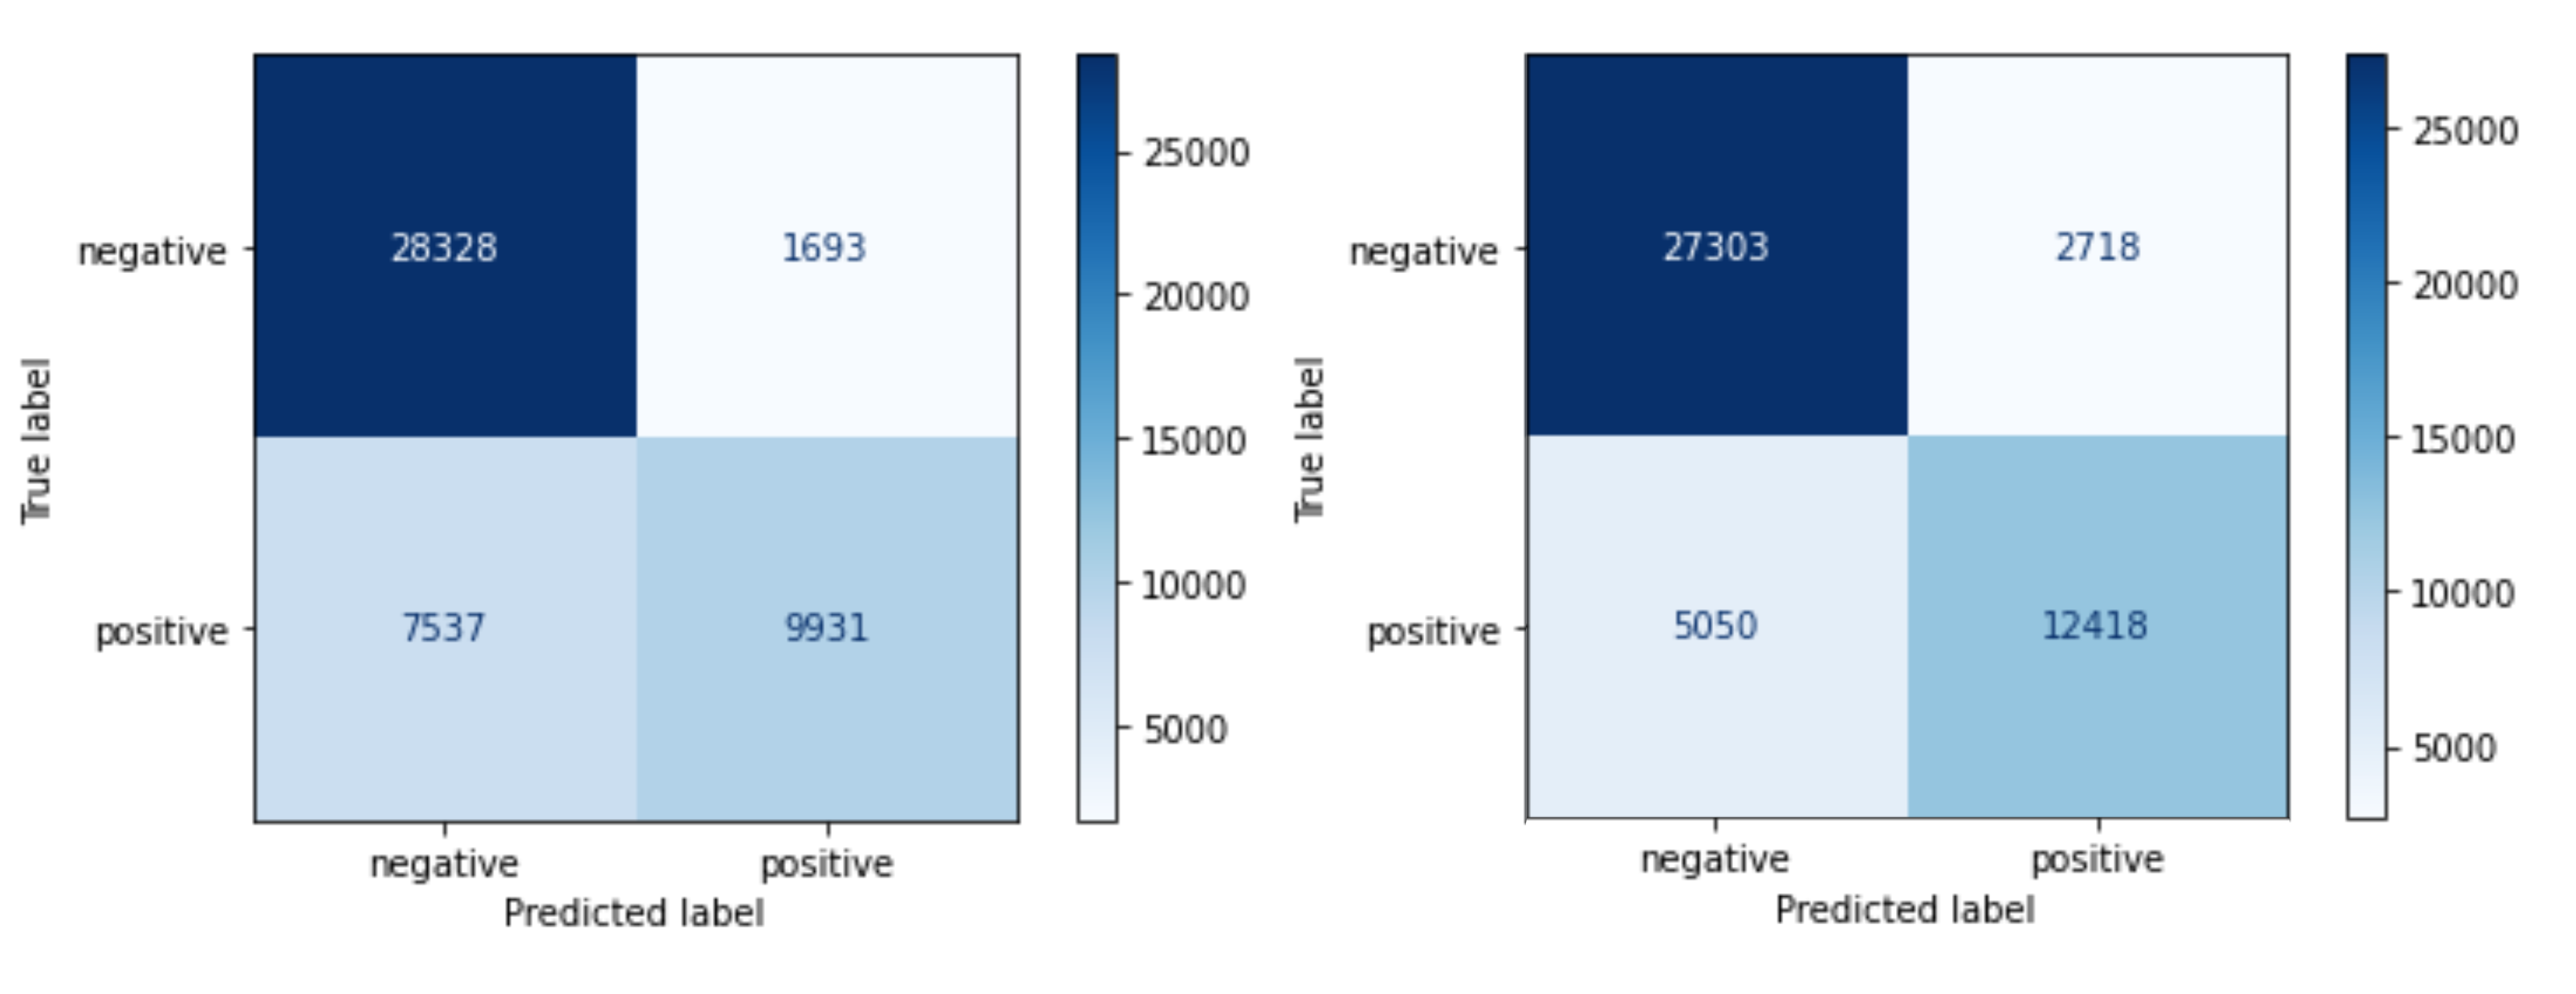
\includegraphics[width=\textwidth]{DME-template/conf_binary.png}
    \caption{SVM vs Logistic Regression for binary classification}
\end{figure}

\begin{figure}[H]
    \centering
    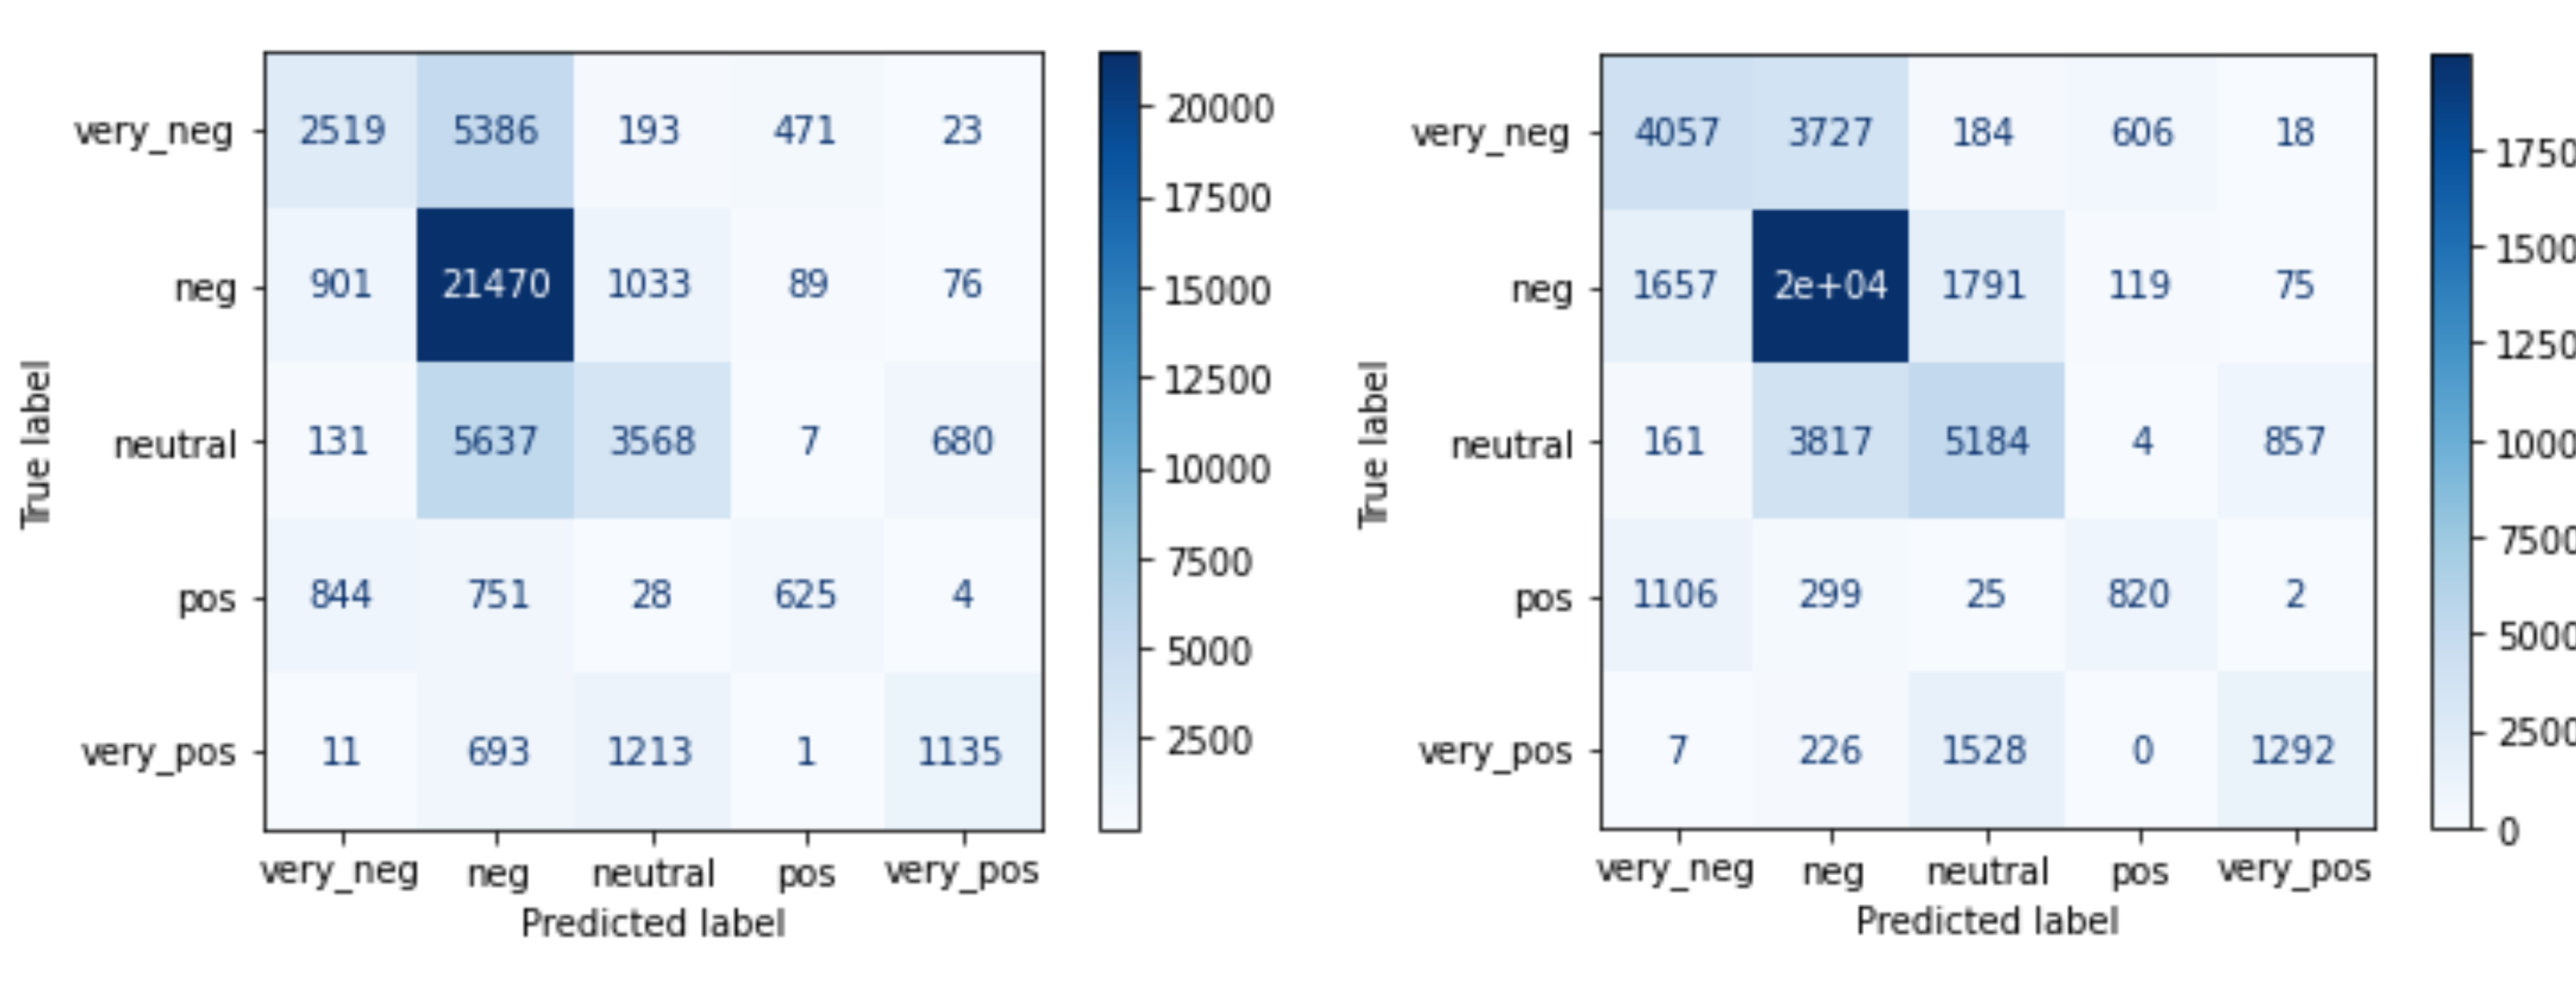
\includegraphics[width=0.7\textwidth]{DME-template/conf_5.png}
    \caption{SVM vs Logistic Regression for multi-label classification}
\end{figure}

% From the classification reports, we can see that Logistic Regression achieved the highest precision in the negative (0.71) and neutral (0.60) classes.

%validation set results



Figure \ref{training_samples} illustrates a significant imbalance among the five classes and the prevalence of class ‘neutral’. Class ‘negative’ accounts for only 4\% of the training set, while class ‘neutral’ covers 49\%. To address the class imbalance issue, we under-sample the predominant class. To understand the effect of sample frequency per class on multi-label classification, we compare our models’ performance before and after under-sampling. The results are shown in Table \ref{tab:undersampled}.

%undersampling

\begin{table}[H]
\centering
\begin{tabular}{|c|cccc|}
\hline
Training-Set     & Precision & Recall  & F1-Score & Accuracy \\ \hline
Normal           & 63.58\%   & 64.97\% & 63.50\%  & 64.97\%  \\
w/ undersampling & 63.62\%   & 63.05\% & 62.48\%  & 63.05\%  \\ \hline
\end{tabular}
\caption{Normal vs under sampled dataset.}
\label{tab:undersampled}
\end{table}




A bag-of-words approach has been shown to have limited performance when trying to predict a `neutral' label for short texts (\cite{wang2012system}). We carried out an experiment in which the labels were reduced by changing the sentiment mapping. Instead of a value in the range (0.4, 0.6] being assigned to `neutral', the `negative' and `positive' labels were made larger. A phrase given a value in the interval (0.2, 0.55] was labelled as `negative', and the interval (0.55, 0.8] was labelled as `positive'. The results of the logistic regression model are shown in Table \ref{tab:4label}.

\begin{table}[H]
\centering
\begin{tabular}{|cccc|}
\hline
Precision & Recall  & F1-Score & Accuracy \\ \hline
72.33\%   & 73.62\% & 72.45\%  & 73.62\%  \\ \hline
\end{tabular}
\caption{Performance of model on 4-label classification}
\label{tab:4label}
\end{table}

%test set results for Logistic Regression
Finally, the generalisation performance of the best-performing model (Logistic Regression with bag-of-words) was evaluated on the held-out test set. The results are shown in Table \ref{tab:final-results}.

\begin{table}[H]
\centering
\begin{tabular}{|cccc|cccc|}
\hline
\multicolumn{4}{|c|}{{\ul 5-label}}       & \multicolumn{4}{c|}{{\ul Binary}}         \\
Precision & Recall  & F1-Score & Accuracy & Precision & Recall  & F1-Score & Accuracy \\ \hline
64.47\%   & 65.78\% & 64.45\%  & 65.78\%  & 83.53\%   & 83.64\% & 83.36\%  & 83.64\%  \\ \hline
\end{tabular}
\caption{Best model (LR BOW) results for 5-label and binary classification on test set.}
\label{tab:final-results}
\end{table}




%4label dataset

\section{Conclusion}
    
In this paper we investigated the effect of two feature representations on the performance of a model performing sentiment analysis. Through numerous experiments we found that a bag-of-words approach yields improved classification performance over a TF-IDF approach. The best-performing model implemented in this work used a logistic regression classifier and achieved an accuracy of 83.2\% for binary sentiment classifications, and 64.97\% for 5-label classification. The model is unable to achieve a high accuracy for multi-class classification, the `neutral' class in particular, has a high misclassification rate. This suggests that the two approaches explored in this paper are not strong enough to accurately classify due to a lack of contextual data within many phrases. More sophisticated feature representations that can capture sentence-level information such as word order are required to achieve high accuracy.


\section{Individual Contributions}

\subsection{Adelina Badea}

My main focus entailed exploring and implementing various supervised learning techniques, such as Logistic Regression, SVM, and Random Forest, for the binary and multi-label classification tasks, using both TF-IDF and BOW representations. Apart from pre-processing the raw data collection, I performed EDA on the resulted classifications, using confusion matrices and ROCs. 

\subsection{Daniel Biró}

During this project I have mostly been contributing to the interpretation of the related works and polishing the reports we have written. I have also took part in examining further unsupervised learning methods other than K-means and attempting to apply them. Other than that I have participated in the general brainstorming about the direction of the project, especially in the beginning when the key parts had to be identified.

\subsection{Azam Khan}
My work in this project involved performing some exploratory data analysis on the dataset and helping with the supervised learning aspect of the project. I setup some experiments, for example, the class undersampling and reduced label experiments, and implemented the LSTM model for both, binary and multi-label classification.

\subsection{Evan Moss}
In this project, I was responsible for the initial exploration of unsupervised learning methods (K-means), as well as the exploratory data analysis section. My particular focus in the EDA section was to find interesting and useful visualisations to present, which would give us an idea of the structure of the data. I was also involved in the pre-processing of the data, including the lemmatisation process.

\bibliographystyle{plainnat}
\bibliography{bibfile}

\end{document}
